\section{Programa de Trabajo}

\subsection{Descripción de las actividades}

\begin{enumerate}
	\item Identificar en conjunto con el experto de ALMA una problemática contingente al análisis de logs.

	\item Definir los requisitos del problema identificado.

	\item En conjunto con el experto de ALMA, establecer características relevantes en los patrones de LOGs.
	
	\item Implementar una herramienta para la representación visual de las secuencias de log.

	\item Abordar la problemática utilizando la literatura relacionada con el tema de análisis de logs.
	
	\item Identificar una técnica adecuada para enfrentar la problemática.
	
	\item Desarrollar un proceso reducido de \textbf{KDD}, sin iteraciones, basándose en la técnica previamente seleccionada.
	\begin{enumerate}
		\item Selección de un set de datos y operaciones de pre-procesamiento sobre los mismos.
		\item Extracción de características de las secuencias.
		\item Procesamiento de los datos.
		\item Validación de los resultados.
	\end{enumerate}
	
	\item Elaboración del proyecto.
	
\end{enumerate}

\subsection{Carta Gantt}

\begin{figure}[H]
\centering
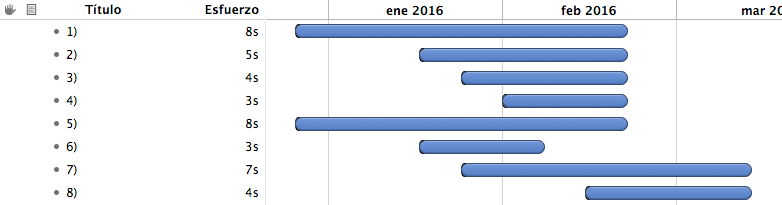
\includegraphics[scale=0.5]{img/gantt}
\caption{Carta Gantt}
\end{figure}

